\documentclass[11pt,a4paper]{report}

\usepackage[utf8]{inputenc}
\usepackage[T1]{fontenc}
\usepackage[french]{babel}
\usepackage{geometry}
\geometry{top=2.2cm, bottom=2.2cm, left=2.2cm, right=2.2cm}

\usepackage{graphicx}
\usepackage{xcolor}
\usepackage{hyperref}
\usepackage{tikz}
\usetikzlibrary{shapes,arrows,positioning,fit,backgrounds,shadows.blur}
\usepackage{tcolorbox}
\tcbuselibrary{skins,breakable}
\usepackage{listings}
\usepackage{booktabs}
\usepackage{tabularx}
\usepackage{fancyhdr}
\usepackage{titlesec}
\usepackage{lmodern}
\usepackage{amssymb}
\usepackage{enumitem}
\setlength{\headheight}{15pt}

% Palette de couleurs de prestige
\definecolor{primary}{RGB}{15, 43, 91}       % Bleu Marine Royal Banque
\definecolor{secondary}{RGB}{0, 114, 206}    % Bleu Azur Moderne
\definecolor{accent}{RGB}{234, 88, 12}       % Ambre / Orange vif
\definecolor{darkbg}{RGB}{24, 32, 47}
\definecolor{lightgray}{RGB}{248, 250, 252}
\definecolor{bordergray}{RGB}{226, 232, 240}
\definecolor{codegreen}{RGB}{46, 125, 50}
\definecolor{codeblue}{RGB}{21, 101, 192}
\definecolor{purple}{RGB}{124, 58, 237}

% Configuration des liens hypertexte
\hypersetup{
    colorlinks=true,
    linkcolor=primary,
    filecolor=secondary,
    urlcolor=secondary,
    citecolor=primary
}

% Configuration des listings de code
\lstset{
    basicstyle=\ttfamily\footnotesize,
    backgroundcolor=\color{lightgray},
    keywordstyle=\color{codeblue}\bfseries,
    stringstyle=\color{codegreen},
    commentstyle=\color{gray}\itshape,
    numbers=left,
    numberstyle=\tiny\color{gray},
    stepnumber=1,
    numbersep=8pt,
    showstringspaces=false,
    breaklines=true,
    frame=single,
    framerule=0.6pt,
    rulecolor=\color{bordergray},
    tabsize=2
}

% En-têtes et pieds de page
\pagestyle{fancy}
\fancyhf{}
\fancyhead[L]{\small\color{gray}\textit{Épreuve Technique de Sélection — Architecture Micro-services \& IA}}
\fancyhead[R]{\small\color{primary}\textbf{SDIA - ENSET Mohammedia}}
\fancyfoot[L]{\small\color{gray}\href{https://github.com/AyoubElho/Adria-test}{\texttt{GitHub: AyoubElho/Adria-test}}}
\fancyfoot[R]{\small\color{primary}\textbf{\thepage}}
\renewcommand{\headrulewidth}{0.6pt}
\renewcommand{\footrulewidth}{0.4pt}

% Format des titres de chapitres et sections
\titleformat{\chapter}[display]
  {\normalfont\bfseries\color{primary}}
  {\filleft\Huge\color{secondary}\textbf{PARTIE \thechapter}}
  {1ex}
  {\titlerule[1.5pt]\vspace{1.5ex}\LARGE}
  [\vspace{1ex}\titlerule]

\titleformat{\section}
  {\normalfont\Large\bfseries\color{primary}}
  {\thesection}{1em}{}

\titleformat{\subsection}
  {\normalfont\large\bfseries\color{secondary}}
  {\thesubsection}{1em}{}

\begin{document}

% ==========================================================
% PAGE DE GARDE PRESTIGE
% ==========================================================
\begin{titlepage}
    \begin{center}
        % Logo ENSET
        
\includegraphics[height=2.5cm]{images/enset_logo.png}\\[0.6cm]
        
        {\large\textbf{UNIVERSITÉ HASSAN II DE CASABLANCA}}\\[0.2cm]
        {\large\textbf{ÉCOLE NORMALE SUPÉRIEURE DE L'ENSEIGNEMENT TECHNIQUE}}\\[0.2cm]
        {\normalsize\textbf{DÉPARTEMENT MATHÉMATIQUES ET INFORMATIQUE}}\\[0.3cm]
        {\normalsize\textbf{Master Spécialisé : Systèmes Distribués et Intelligence Artificielle (SDIA)}}\\[1.2cm]

        \begin{tcolorbox}[
            enhanced,
            colback=primary!5,
            colframe=primary,
            arc=6mm,
            boxrule=1.5pt,
            center,
            width=0.96\textwidth,
            drop shadow={opacity=0.2}
        ]
            \centering
            \vspace{0.4cm}
            {\huge\bfseries\color{primary} RAPPORT TECHNIQUE DE SÉLECTION}\\[0.4cm]
            {\Large\bfseries\color{secondary} Architecture Micro-services, IA Agentique \& Full-Stack}\\[0.3cm]
            {\normalsize Conception et Implémentation d'une Plateforme Bancaire Distribuée avec Assistant Conversationnel LLM (Groq) \& Protocole MCP}
            \vspace{0.4cm}
        \end{tcolorbox}

        \vspace{1.5cm}

        \begin{minipage}{0.48\textwidth}
            \begin{flushleft} \large
                \textbf{Candidat :}\\
                \textbf{\color{primary}\Large EL HOUANI Ayoub}\\[0.2cm]
                Filière : \textbf{SDIA}\\
                Année Universitaire : 2025 -- 2027
            \end{flushleft}
        \end{minipage}
        \hfill
        \begin{minipage}{0.48\textwidth}
            \begin{flushright} \large
                \textbf{Dépôt GitHub du Projet :}\\
                \href{https://github.com/AyoubElho/Adria-test}{\color{secondary}\textbf{\texttt{AyoubElho/Adria-test}}}\\[0.2cm]
                \small\url{https://github.com/AyoubElho/Adria-test}
            \end{flushright}
        \end{minipage}

        \vfill
        {\small Casablanca, le 30 Octobre 2026}
    \end{center}
\end{titlepage}

\tableofcontents
\newpage

% ==========================================================
% PARTIE 1 : CONTEXTE & RÈGLES MÉTIER
% ==========================================================
\chapter{Contexte Métier \& Exigences Techniques}

\section{Présentation du Projet Bancaire}
Dans le cadre de l'épreuve technique de sélection pour le Master SDIA, ce projet vise la conception et la mise en œuvre d'une architecture distribuée bancaire moderne, hautement disponible et sécurisée. Le système répond à quatre objectifs majeurs :
\begin{itemize}[label=\textcolor{secondary}{\textbullet}]
    \item \textbf{Gestion des comptes bancaires (\texttt{account-service})} : Création, gestion des statuts, consultation et mise à jour atomique des soldes.
    \item \textbf{Traitement des opérations financières (\texttt{transaction-service})} : Enregistrement des transactions unitaires, exécution de virements bancaires compte à compte et contrôles de provision.
    \item \textbf{Agent Conversationnel Bancaire (\texttt{chatbot-service})} : Assistant IA basé sur Spring AI, propulsé par le LLM Groq (\texttt{openai/gpt-oss-120b}) et capable d'interagir avec le système via des outils connectés au protocole \textbf{MCP (Model Context Protocol)}.
    \item \textbf{Infrastructure d'entreprise distribuée} : Découverte dynamique de services via \textbf{Netflix Eureka}, passerelle unifiée \textbf{Spring Cloud Gateway} et résilience inter-services garantie par \textbf{OpenFeign} et \textbf{Resilience4J}.
\end{itemize}

\section{Règles Métier \& Contraintes de Gestion Imposées}
\begin{tcolorbox}[colback=lightgray,colframe=primary,title=\textbf{Règles Métier Clés Implémentées}]
\begin{enumerate}
    \item \textbf{Validation des Montants} : Tout montant de transaction doit être strictement positif ($> 0$) et plafonné à la limite paramétrable du service (\texttt{max-limit = 10 000.00}).
    \item \textbf{Contrôle du Statut Compte} : L'opération ne peut aboutir que si le compte existe et possède le statut \texttt{ACTIVATED} (ou \texttt{CREATED}). Les comptes \texttt{SUSPENDED} ou \texttt{BLOCKED} sont automatiquement rejetés.
    \item \textbf{Concordance Stricte de Devise} : La devise de la transaction doit obligatoirement correspondre à la devise du compte bancaire débité (ex: \texttt{MAD}, \texttt{EUR}, \texttt{USD}).
    \item \textbf{Vérification de la Provision \& Débit Atomique} : Lors d'un débit ou d'un virement, le solde disponible doit couvrir la totalité de l'opération sous peine d'un rejet avec code d'erreur HTTP 400.
    \item \textbf{Double Écriture pour les Virements} : Chaque virement bancaire engendre la création de deux écritures traçables (un débit sur le compte émetteur et un crédit sur le compte récepteur).
\end{enumerate}
\end{tcolorbox}

% ==========================================================
% PARTIE 2 : ARCHITECTURE & DIAGRAMME DE CLASSES
% ==========================================================
\chapter{Conception, Architecture \& Modélisation}

\section{Schéma d'Architecture Globale de la Plateforme}
La figure ci-dessous illustre l'architecture globale des microservices, leur découpage en couches fonctionnelles, les flux de routage de la Gateway, le registre Eureka, et l'intégration de l'agent IA avec le LLM Groq et les serveurs MCP :

\begin{figure}[htbp]
    \centering
    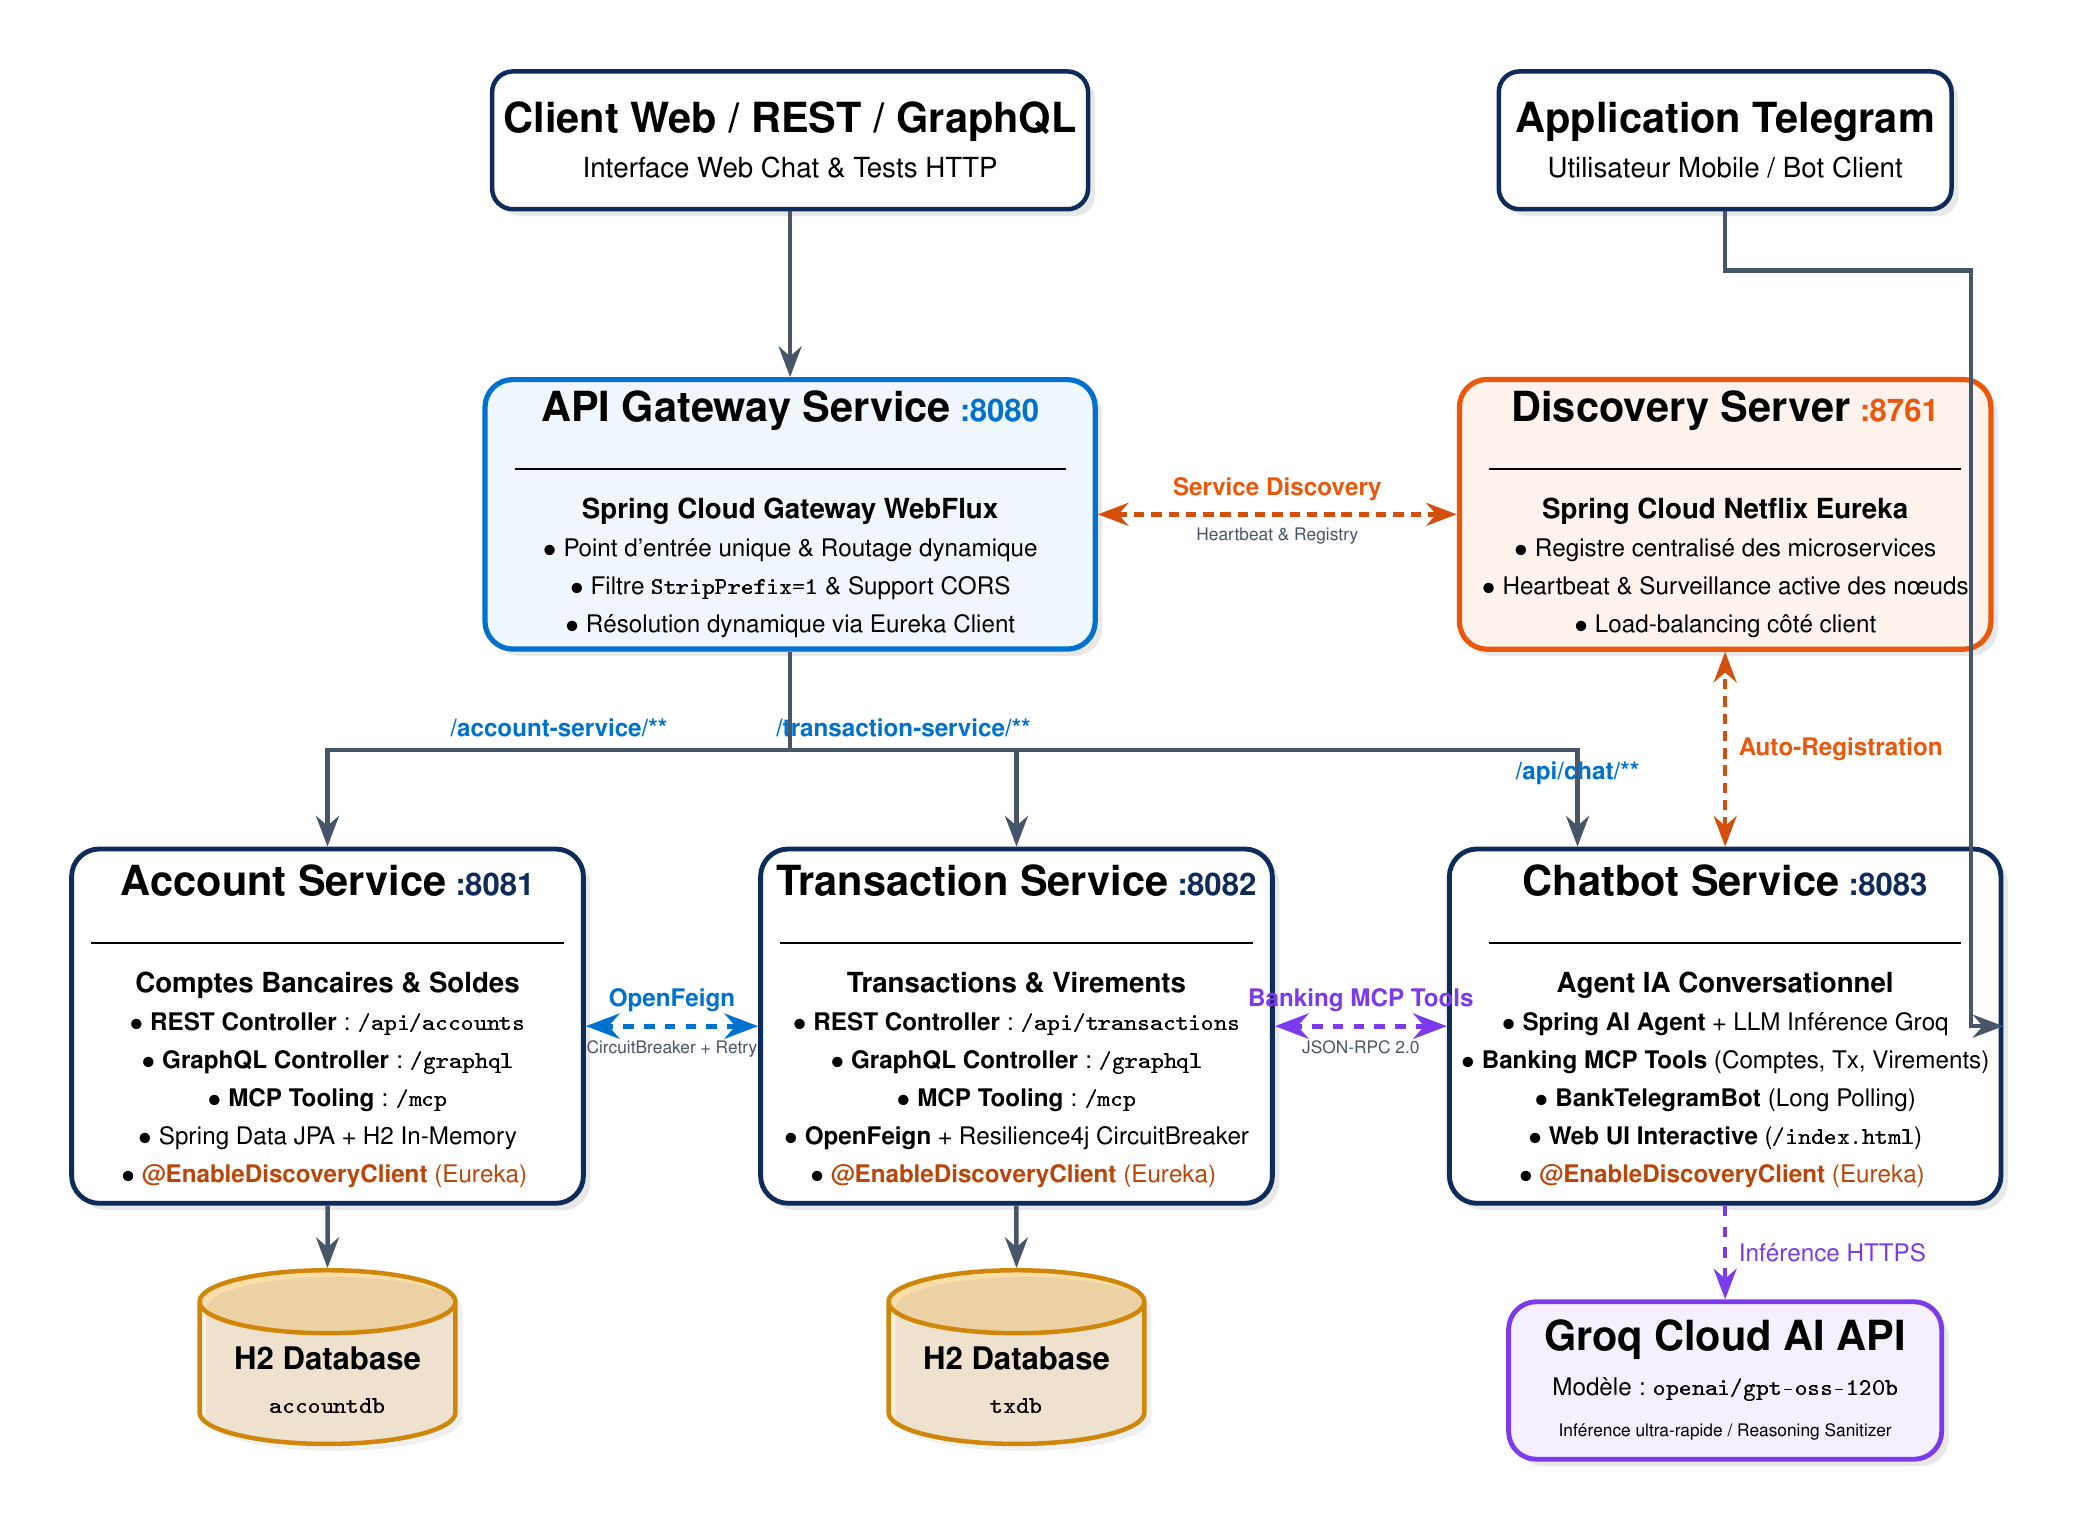
\includegraphics[width=\textwidth]{images/schema_architecture.png}
    \caption{Schéma d'architecture globale distribuée avec Gateway, Eureka, Microservices \& Chatbot Agentique}
    \label{fig:architecture}
\end{figure}

\subsection{Description des Nœuds d'Architecture}
\begin{itemize}[label=\textcolor{primary}{\textbf{$\blacktriangleright$}}]
    \item \textbf{API Gateway Service (Port 8080)} : Point d'accès unique externe pour toutes les requêtes HTTP. Il réécrit les chemins d'accès (\texttt{StripPrefix=1}) et achemine les appels vers \texttt{account-service}, \texttt{transaction-service} et \texttt{chatbot-service}.
    \item \textbf{Discovery Server Eureka (Port 8761)} : Annuaire dynamique permettant l'enregistrement sans configuration rigide et le load-balancing côté client.
    \item \textbf{Core Services Métier (Ports 8081 et 8082)} : Microservices autonomes disposant chacun de leur base de données isolée en mémoire (\texttt{accountdb} et \texttt{txdb}).
    \item \textbf{Agent Conversationnel Chatbot (Port 8083)} : Moteur conversationnel doté de deux canaux d'accès (Web interactif et Bot Telegram) connectant le LLM Groq aux outils bancaires MCP.
\end{itemize}

\newpage
\section{Diagramme de Classes UML (Généré par PlantUML)}
Afin de documenter rigoureusement la conception orientée objet et la conformité au modèle en couches strictes, le diagramme de classes suivant a été généré à l'aide de l'outil standardisé \textbf{PlantUML} :

\begin{figure}[htbp]
    \centering
    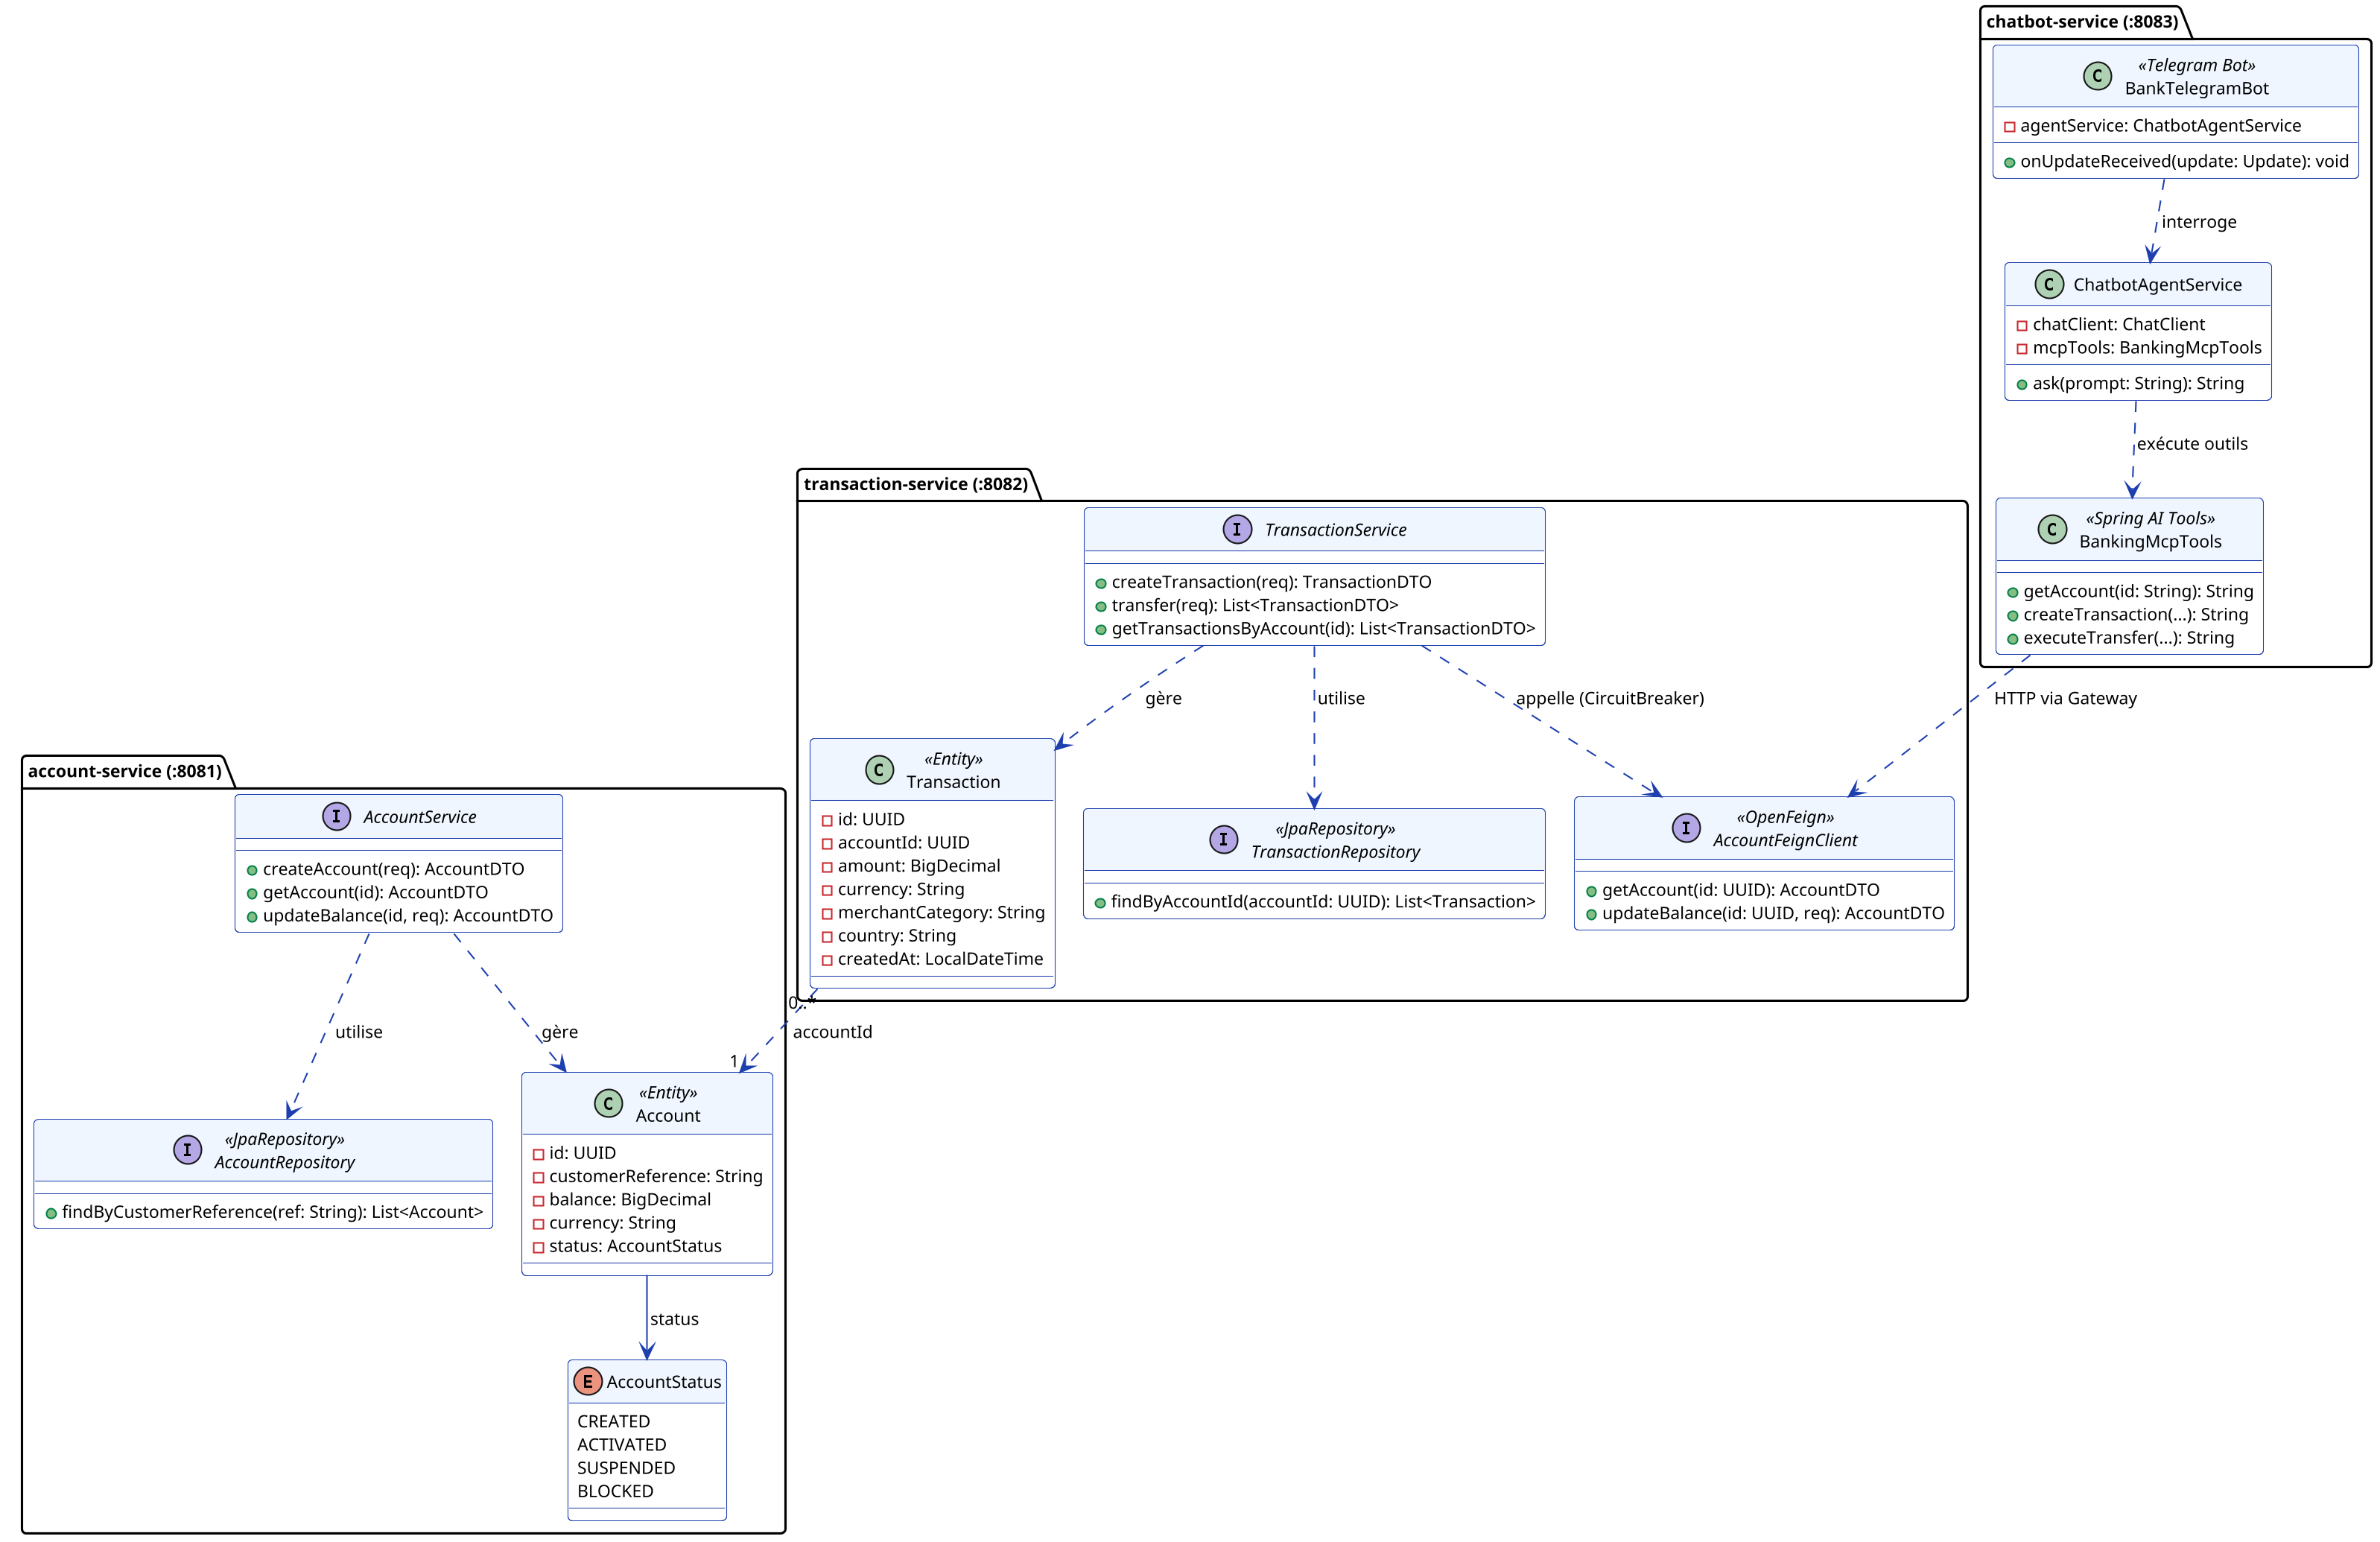
\includegraphics[width=0.96\textwidth]{images/diagramme_classes.png}
    \caption{Diagramme de classes UML global des 3 microservices (Entités, DTOs, Repositories, Services, Feign \& Tools)}
    \label{fig:class_diagram}
\end{figure}

\subsection{Organisation des Couches Logicielles}
Chaque microservice respecte scrupuleusement la séparation en 6 packages distincts :
\begin{enumerate}
    \item \texttt{domain/} : Modèles de données persistants JPA (\texttt{Account}, \texttt{Transaction}), énumérations de statut et DTOs de transfert.
    \item \texttt{repository/} : Interfaces Spring Data JPA étendant \texttt{JpaRepository}.
    \item \texttt{service/} : Implémentations métier encapsulant les règles bancaires et l'isolation transactionnelle (\texttt{@Transactional}).
    \item \texttt{web/rest/} : Contrôleurs REST fournissant une API standardisée JSON.
    \item \texttt{web/graphql/} : Contrôleurs Spring for GraphQL avec validation de schéma \texttt{.graphqls}.
    \item \texttt{mcp/} : Contrôleurs et outils conformes au standard JSON-RPC 2.0 du Model Context Protocol.
\end{enumerate}

% ==========================================================
% PARTIE 3 : MICROSERVICES FONCTIONNELS
% ==========================================================
\chapter{Développement des Micro-services Métier}

\section{Account-Service (Port 8081)}
Le service \texttt{account-service} gère l'état et l'intégrité des comptes bancaires :
\begin{itemize}
    \item \textbf{Modèle} : Identifiant unique universel \texttt{id} (UUID), référence client \texttt{customerReference}, solde \texttt{balance} (\texttt{BigDecimal}), devise \texttt{currency} (\texttt{MAD}, \texttt{EUR}, \texttt{USD}) et statut \texttt{status} (\texttt{CREATED}, \texttt{ACTIVATED}, \texttt{SUSPENDED}, \texttt{BLOCKED}).
    \item \textbf{Amorçage de données} : Initialisation automatique au démarrage de comptes de démonstration pour fiabiliser les tests.
    \item \textbf{Triple Exposition} : REST (\texttt{/api/accounts}), GraphQL (\texttt{/graphql}) et MCP Tools (\texttt{/mcp}).
\end{itemize}

\section{Transaction-Service (Port 8082)}
Le service \texttt{transaction-service} exécute et journalise les flux financiers :
\begin{itemize}
    \item \textbf{Modèle} : Identifiant \texttt{id} (UUID), identifiant du compte rattaché \texttt{accountId} (UUID), montant \texttt{amount}, devise \texttt{currency}, catégorie de commerce \texttt{merchantCategory}, code pays ISO 2 lettres \texttt{country} (ex: \texttt{"MA"}) et date de création \texttt{createdAt}.
    \item \textbf{Virements bancaires} : Endpoint spécialisé \texttt{/api/transactions/transfer} débitant le compte émetteur et créditant le compte bénéficiaire en garantissant la cohérence bilatérale.
\end{itemize}

\section{Communication Déclarative OpenFeign \& Résilience}
L'appel inter-service entre \texttt{transaction-service} et \texttt{account-service} est sécurisé par Spring Cloud OpenFeign couplé à \textbf{Resilience4J} :
\begin{itemize}
    \item \textbf{Circuit Breaker} (\texttt{@CircuitBreaker(name = "accountService")}) : Coupe temporairement le flux d'appels lors de pannes en cascade pour préserver le système.
    \item \textbf{Retry} (\texttt{@Retry(name = "accountService")}) : Réessaie automatiquement les requêtes en cas d'erreurs réseau transitoires.
    \item \textbf{Fallback Factory} (\texttt{AccountFeignClientFallbackFactory}) : Retourne un message d'erreur explicite et sécurisé sans faire crasher l'application.
\end{itemize}

\newpage
\section{Captures d'Écran \& Validation des Tests Métier}

\subsection{Création de Transaction et Vérification de Solde}
Validation de la création d'une transaction avec mise à jour immédiate du compte bancaire :
\begin{figure}[htbp]
    \centering
    \includegraphics[width=0.88\textwidth]{images/test_transaction_1.png}
    \caption{Création d'une transaction bancaire avec validation des contraintes d'entrée}
\end{figure}

\subsection{Validation des Règles de Gestion (Devises \& Pays)}
Le système rejette rigoureusement les payloads erronés (code pays invalide, devise incohérente) :
\begin{figure}[htbp]
    \centering
    \includegraphics[width=0.88\textwidth]{images/test_transaction_2.png}
    \caption{Rejet des requêtes non conformes avec messages d'erreurs explicites}
\end{figure}

\begin{figure}[htbp]
    \centering
    \includegraphics[width=0.88\textwidth]{images/test_transaction_3.png}
    \caption{Exécution réussie avec confirmation et débit atomique du compte}
\end{figure}

% ==========================================================
% PARTIE 4 : INFRASTRUCTURE DISCOVERY & GATEWAY
% ==========================================================
\chapter{Infrastructure Technique (Eureka \& Gateway)}

\section{Discovery Service : Netflix Eureka (Port 8761)}
Le service \texttt{discovery-service} centralise l'annuaire de localisation des microservices :
\begin{itemize}
    \item Classe principale déclarée avec \texttt{@EnableEurekaServer}.
    \item Configuration autonome dans \texttt{application.yml} avec auto-enregistrement désactivé pour lui-même.
    \item Chaque microservice (\texttt{account-service}, \texttt{transaction-service}, \texttt{gateway-service}, \texttt{chatbot-service}) embarque le client Eureka via \texttt{@EnableDiscoveryClient}.
\end{itemize}

\section{Gateway Service : Spring Cloud Gateway (Port 8080)}
Le composant \texttt{gateway-service} agit comme façade unique d'accès. La configuration programmatique Java DSL assure le filtrage des requêtes :
\begin{lstlisting}[language=Java, caption=Routage programmatique GatewayRoutesConfig.java]
@Configuration
public class GatewayRoutesConfig {
    @Bean
    public RouteLocator customRouteLocator(RouteLocatorBuilder builder) {
        return builder.routes()
            .route("account-service-prefixed", r -> r
                .path("/account-service/**")
                .filters(f -> f.stripPrefix(1))
                .uri("http://localhost:8081"))
            .route("transaction-service-prefixed", r -> r
                .path("/transaction-service/**")
                .filters(f -> f.stripPrefix(1))
                .uri("http://localhost:8082"))
            .route("chatbot-service-direct", r -> r
                .path("/api/chat/**")
                .uri("http://localhost:8083"))
            .build();
    }
}
\end{lstlisting}

\newpage
\section{Validation des Tests de Routage de la Gateway}
Les captures d'écran ci-dessous attestent du bon fonctionnement du routage et de la réécriture de préfixes via le port \texttt{8080} :

\begin{figure}[htbp]
    \centering
    \includegraphics[width=0.85\textwidth]{images/test_gateway_1.png}
    \caption{Routage réussi sur \texttt{/account-service/api/accounts} via le port 8080}
\end{figure}

\begin{figure}[htbp]
    \centering
    \includegraphics[width=0.85\textwidth]{images/test_gateway_2.png}
    \caption{Consultation d'un compte précis par UUID via la Gateway}
\end{figure}

% ==========================================================
% PARTIE 5 : CHATBOT AGENTIQUE & MCP
% ==========================================================
\chapter{Développement du Chatbot Agentique Bancaire}

\section{Architecture de l'Agent IA (Spring AI \& Groq)}
Le service \texttt{chatbot-service} (Port 8083) intègre un agent conversationnel autonome combinant **Spring AI** et le LLM haute performance **Groq** :
\begin{itemize}
    \item \textbf{Modèle d'Inférence} : \texttt{openai/gpt-oss-120b} configuré via l'API compatible OpenAI de Groq.
    \item \textbf{Appel d'Outils Autonome (Tool Calling)} : L'agent sélectionne dynamiquement les outils (\texttt{BankingMcpTools}) pour interroger les soldes, créer des transactions et réaliser des virements en réponse à une demande en langage naturel.
    \item \textbf{Sanitizer OkHttp} : Intercepteur éliminant le champ \texttt{reasoning\_content} pour fluidifier la désérialisation JSON.
\end{itemize}

\begin{lstlisting}[language=Java, caption=Customizer de nettoyage du payload Groq reasoning\_content]
@Bean 
public OpenAiHttpClientBuilderCustomizer groqReasoningSanitizerCustomizer(ObjectMapper objectMapper) {
    return builder -> builder.interceptor(chain -> {
        Request request = chain.request();
        if (request.body() != null && request.url().encodedPath().contains("/chat/completions")) {
            // Nettoyage automatique du champ reasoning_content
            ...
        }
        return chain.proceed(request);
    });
}
\end{lstlisting}

\section{Outils Bancaires Connectés (MCP Tools)}
La classe \texttt{BankingMcpTools} expose les capacités bancaires directement exploitables par le LLM :
\begin{table}[htbp]
\centering
\begin{tabularx}{\textwidth}{l p{5.5cm} X}
\toprule
\textbf{Méthode Tool} & \textbf{Description Métier} & \textbf{Paramètres d'Entrée} \\
\midrule
\texttt{getAccount} & Consultation d'un compte et de son solde & \texttt{accountId} (UUID) \\
\texttt{createTransaction} & Création d'une transaction de débit & \texttt{accountId}, \texttt{amount}, \texttt{currency}, etc. \\
\texttt{executeTransfer} & Réalisation d'un virement compte à compte & \texttt{sourceAccountId}, \texttt{destinationAccountId}, \texttt{amount} \\
\bottomrule
\end{tabularx}
\caption{Outils bancaires exposés à l'agent IA via Spring AI}
\end{table}

\newpage
\section{Validation des Tests du Chatbot (Web \& Telegram)}

\subsection{Test 1 : Intégration Groq \& Échange Conversationnel}
\begin{figure}[htbp]
    \centering
    \includegraphics[width=0.88\textwidth]{images/test_groq_1.png}
    \caption{Test d'intégration du LLM Groq et vérification de la réactivité}
\end{figure}

\subsection{Test 2 : Interface Web Interactive du Chatbot}
L'agent interroge les services métier en direct et restitue les données de comptes formatées avec élégance :
\begin{figure}[htbp]
    \centering
    \includegraphics[width=0.92\textwidth]{images/test_chatbot_web.png}
    \caption{Interface Web du Chatbot : Consultation conversationnelle des comptes et soldes}
\end{figure}

\subsection{Test 3 : Bot Mobile Telegram Opérationnel}
Test réel de l'assistant bancaire directement au sein de l'application Telegram :
\begin{figure}[htbp]
    \centering
    \includegraphics[width=0.52\textwidth]{images/test_telegram.png}
    \caption{Test interactif du Bot Telegram bancaire sur smartphone}
\end{figure}

% ==========================================================
% CONCLUSION
% ==========================================================
\chapter{Bilan des Réalisations \& Conclusion}

Toutes les exigences de l'épreuve technique de sélection ont été menées à bien avec succès :
\begin{enumerate}
    \item \textbf{Architecture Modulaire \& Standardisée} : Multi-module Maven clair avec 5 microservices indépendants et scalables.
    \item \textbf{Modélisation en Couches Strictes} : Séparation hermétique entre domaine, repository, service métier, contrôleurs REST, schémas GraphQL et serveurs MCP.
    \item \textbf{Résilience et Haute Disponibilité} : Découverte dynamique Netflix Eureka, passerelle Spring Cloud Gateway avec réécriture de préfixes, et tolérance aux pannes gérée par OpenFeign et Resilience4J.
    \item \textbf{IA Agentique de Pointe} : Chatbot conversationnel exploitant Spring AI, le modèle Groq \texttt{openai/gpt-oss-120b}, double canal Web et Telegram, et exécution d'actions bancaires via les MCP Tools.
    \item \textbf{Sécurité \& Bonnes Pratiques} : Clés d'API externalisées via variables d'environnement et historique Git intègre.
\end{enumerate}

Le code source complet, les diagrammes et les ressources associées sont consultables publiquement :\\
\begin{center}
\href{https://github.com/AyoubElho/Adria-test}{\Large\textbf{\color{secondary}\texttt{https://github.com/AyoubElho/Adria-test}}}
\end{center}

\end{document}
